\documentclass [11pt]{article}

\usepackage{amsmath}
\usepackage{amsfonts}
\usepackage{amssymb}
\usepackage{graphicx}
\usepackage{subcaption}
\usepackage{float}
\usepackage{fancyvrb}



\title{FYS-STK4155 Mandatory Assignment 1: \\ Regression analysis and resampling methods}
\author{Minh Chien Nguyen (davidngcz@gmail.com)}

\begin{document}
\maketitle
\nocite{*}
\begin{abstract}
The aim of this project is to compare three traditional approaches to regression analysis: Ordinary Least Squares method, Ridge regression and Lasso regression, using both simulated data and real data. In order to perform a proper assessment of the presented techniques, we employ a statistical method called k-fold cross-validation. Our results reveal that for models with small number of included features the OSL regression method outperforms the more complex methods using regularization in nearly every aspect considered. In addition, we conclude that regression methods in the form we present here are not a suitable approach for performing data analysis of larger datasets.
\end{abstract}

\section*{Introduction}
Regression is the oldest, simple and widely used supervised machine learning algorithm for data analysis. This method is mostly used for forecasting and finding out a relationship between variables. The difference between regression techniques is based on the number of independent variables and the type of relationship between the independent and dependent variables. Here, we will restrict ourselves to the case of polynomial regression.\\
\\
Three traditional methods of regression are recognized: Ordinary Least Squares method, Ridge regression and Lasso regression. All of them have received much attention among practitioners, as well as in academic literature.\\
\\
This text is organized as follows. Main tools and results which allow for application to fitting functions are presented in Section \ref{sec:techniques}. We further test the performance of the presented methods on a Franke's
function. Finally, the techniques are applied to real data in Section \ref{sec:realdata}. In the last part of the text, we resume the principal results and suggest potential improvements in the future.
\section{Mathematical tools}
\label{sec:techniques}
This section provides an overview of basic regression methods. Preliminary knowledge of statistic is expected. There are many excellent textbooks (see e. g. \cite{abc},\cite{TRJ} and \cite{def}) which cover these topics. Here, however, the subtle mathematical issues are not addressed and we will present the main tools and results without details, but it will suffice for immediate application to fitting functions.\\

\subsection{Simple Linear Regression - Ordinary Least Squares}
Linear regression is the most widely used statistical technique for predictive modeling since it is very simple and often provides a good description of how the inputs affect the output.\\
Let $(x_{1},y_{1}),\ldots,(x_{N},y_{N})$ to be observed data, where each $x_{i} = (x_{i1},x_{i2},\ldots,x_{i p})$ is a vector obtained from the $i\text{th}$ measurement. The set of variables $(x_{1},\ldots,x_{N})$ is called the independent variable or the predictor variable while the set of variable $y=(y_{1},\ldots,y_{N})$ is called the dependent or the response variable. \\
The goal of the regression analysis is to extract or exploit relationship between variables $y_i$ and $x_i$. The linear regression model assumes that there exists $\beta=(\beta_{0},\beta_{1},\ldots,\beta_{p})^{T}$ satisfying 
\begin{equation}
y_{i}=f(x_{i})=\beta_{0} + \sum_{j=1}^{p}x_{ij}\beta_{j}.
\end{equation}
The method of the ordinary least squares (OLS) suggest that the coefficients $\beta$ should minimize the residual sum of squares
\begin{equation}
\hat{\beta}=\text{argmin}_{\beta} ( \sum_{i=1}^{N}(y_{i}- \beta_{0}- \sum_{j=1}^{p}x_{ij}\beta_{j})^{2}).
\label{eq:ols}
\end{equation}
The unique solution to equation \eqref{eq:ols} is given by (see \cite{def})
\begin{equation}
\hat{\beta} =\left(\hat{X}^T\hat{X}\right)^{-1}\hat{X}^T\hat{y}.
\end{equation}

\subsection{Regularization}
One of the common problem while using OLS model is overfitting, which means that the model contains more parameters that can be justified by data. To solve the problem of overfitting in our model we need to increase the flexibility of our model by using regularization. The main concept behind this approach is simplifying the model as much as possible. In other words, we reduce the magnitude of the coefficients of inputs in our model. In the following part, we present two different types of regression techniques using regularization. For more general discussions we refer to \cite{abc}.

\subsubsection*{Ridge Regression}
The first techniques is called ridge regression and its coefficients are defined by \cite{TRJ}
\begin{equation}
\hat{\beta}^{\text{ridge}}=\text{argmin}_{\beta} ( \sum_{i=1}^{N}(y_{i}- \beta_{0}- \sum_{j=1}^{p}x_{ij}\beta_{j})^{2}+ \alpha \sum_{j=1}^{p} \beta_{j}^{2}).
\label{eq:ridge}
\end{equation}
In equation \eqref{eq:ridge} we added an extra term, which is known as the penalty term. $\alpha \geq 0$ is called tuning parameter. It easy to see that higher the value of $\alpha$, higher is the term 
\begin{equation*}
\sum_{i=1}^{N}(y_{i}- \beta_{0}- \sum_{j=1}^{p}x_{ij}\beta_{j})^{2}+ \alpha \sum_{j=1}^{p} \beta_{j}^{2}
\end{equation*}
therefore the magnitude of coefficients $\beta$ are reduced. Roughly speaking, we punish the cost function for high values of $\beta$. It is important to note that the parameter $\alpha$ can be learned as well. The ridge regression solution is given by
\begin{equation}
\hat{\beta} =\left(\hat{X}^T\hat{X} + \alpha I \right)^{-1}\hat{X}^T\hat{y},
\end{equation}
where $I$ is the $p \times p$ identity matrix.
\subsubsection*{Lasso Regression}
Lasso is similar to ridge, but with a small twist. The lasso estimate is in the form \cite{TRJ}
\begin{equation}
\hat{\beta}^{\text{lasso}}=\text{argmin}_{\beta} ( \sum_{i=1}^{N}(y_{i}- \beta_{0}- \sum_{j=1}^{p}x_{ij}\beta_{j})^{2}+ \alpha \sum_{j=1}^{p} |\beta_{j}|).
\label{eq:lasso}
\end{equation}
An important note to notice in equation \eqref{eq:lasso} is that the only difference from ridge regression is term $\alpha \sum_{j=1}^{p} |\beta_{j}|$. Here, the method might include fewer predictors in the model, since lasso sets the irrelevant coefficient $\beta$ to zero.
\subsection{K-folds cross-validation}
\label{sec_kcross}
K-folds cross-variation is a very useful technique for calculating the performance of prediction models. The general procedure can be described as follows:
\begin{enumerate}
\item Shuffle the dataset randomly.
\item Divide the dataset into k groups.
\item For each group:
\begin{enumerate}
\item Take the group as a test data set.
\item Take the remaining groups as a training data set.
\item Fit a model on the training set and evaluate it on the test set.
\item Calculate the evaluation score.
\end{enumerate}
\item Estimate the accuracy of the model by averaging the evaluation score derived in all the $k$ cases.
\end{enumerate}
For more information about cross-validation, we refer to \cite{TRJ} and \cite{2018arXiv180308823M}.

\subsection{Performance criteria}
To test the performance of our results, we list the relevant criteria that we use throughout this text. In the following part, we will denote $\tilde{y}_i$  the predicted value of the $i-th$ sample and $y_i$ denotes the corresponding true value.\\
\begin{enumerate}
\item Mean squared error (MSE) - measures the average of the squares of the errors, which is defined as
\begin{equation}
MSE(\hat{y},\hat{\tilde{y}}) = \frac{1}{n}
\sum_{i=0}^{n-1}(y_i-\tilde{y}_i)^2,
\end{equation}
it is clear that the smaller the value of MSE, the better the fit.
\item Coefficient of determination $R^{2}$ - is a number that indicates the proportion of the variance in the dependent variable that is predictable from the independent variable. The $R^2$ is defined as
\begin{equation}
R^2(\hat{y}, \tilde{\hat{y}}) = 1 - \frac{\sum_{i=0}^{n - 1} (y_i - \tilde{y}_i)^2}{\sum_{i=0}^{n - 1} (y_i - \bar{y})^2},
\end{equation}
where the mean value of the vector $\hat{y}$ is defined as $\bar{y} =  \frac{1}{n} \sum_{i=0}^{n - 1} y_i$.
\item Bias - is the difference between the expected prediction of our model and the correct value which we want to predict. Bias is defined as
\begin{equation}
Bias^2= \sum_i (f(\boldsymbol{x}_i)-E_\mathcal{L}[\hat{g}_\mathcal{L}(\boldsymbol{x}_i)])^2,
\end{equation}
where $E_{\mathcal{L}}$ denotes the expected value of the functional over the dataset $\mathcal{L}=\{\mathcal{L}_1,
\mathcal{L}_2, \ldots \}$.
\item Variance - is an error from sensitivity to small fluctuation in the training set.
\begin{equation}
Var=\sum_i E[( \hat{g}(\boldsymbol{x}_i)-E[\hat{g}(\boldsymbol{x}_i)])^2],
\end{equation}
models with high variance usually perform very well on training data but have high error on test data.
\end{enumerate}
\section{Testing on simulated and real data}
After the theoretical considerations of the previous sections, we now want to test the performance of the presented techniques. First, we study how to fit polynomials to a Franke's function. Then we apply the methods to the polynomial approximation of digital terrain data.
\subsection{Franke's function}
\label{sebsec:franke}
In this section we perform a regression analysis of a specific two-dimensional function called Franke's
function which is defined for $x,y\in [0,1]$ as

\begin{align}
f(x,y) &= \frac{3}{4}\exp{\left(-\frac{(9x-2)^2}{4} - \frac{(9y-2)^2}{4}\right)}+\frac{3}{4}\exp{\left(-\frac{(9x+1)^2}{49}- \frac{(9y+1)}{10}\right)} \\
&+\frac{1}{2}\exp{\left(-\frac{(9x-7)^2}{4} - \frac{(9y-3)^2}{4}\right)} -\frac{1}{5}\exp{\left(-(9x-4)^2 - (9y-7)^2\right) }.
\label{eq:franke}
\end{align}

Figure \ref{fig:Franke} shows a three-dimensional plot of the Franke's function with an added stochastic noise to it using  the normal distribution $N(0,1)$. From equation \eqref{eq:franke} we know that the Franke's function is a weighted sum of four exponentials and it is clearly an infinitely differentiable function on $[0,1] \times [0,1]$. Therefore, to perform a regression analysis of this function, we will test
polynomial fits in $x$ and $y$ up to fifth order.
\begin{figure}[H]
\centering
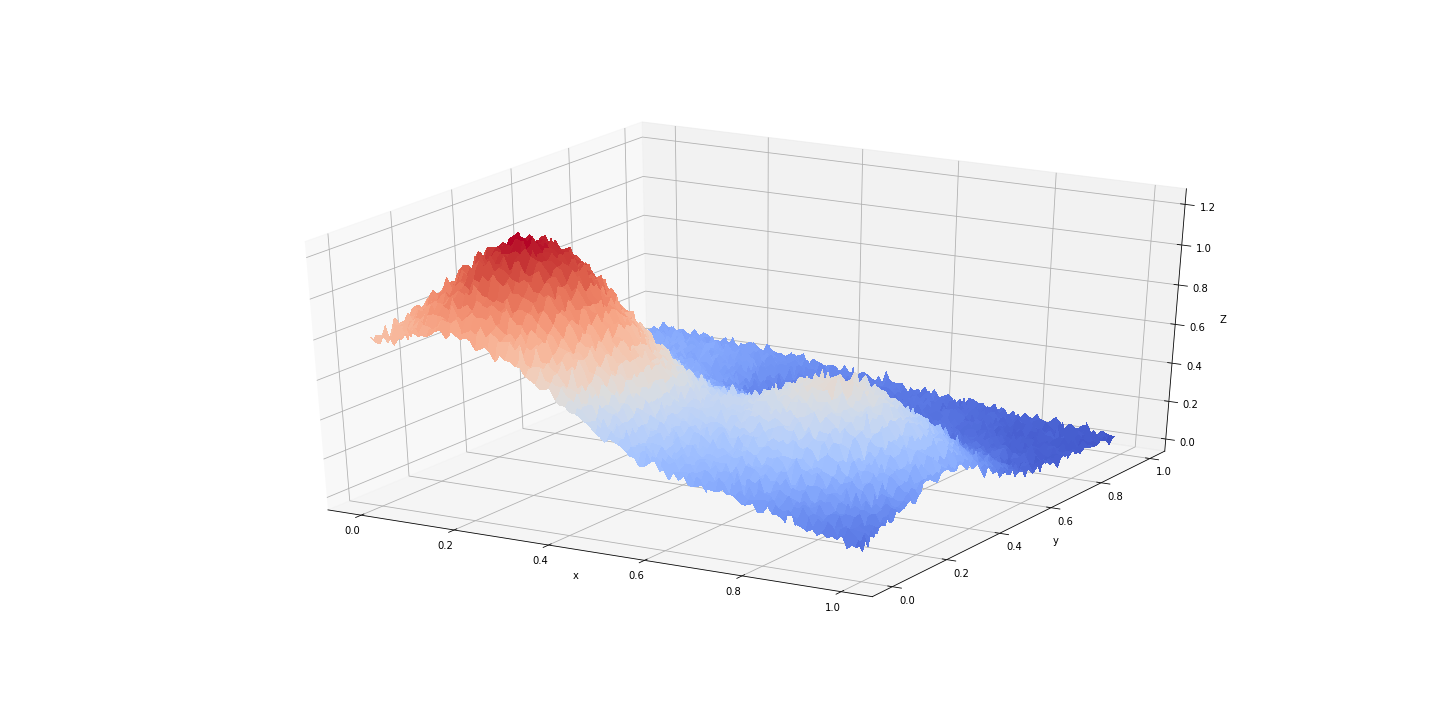
\includegraphics[width=1\textwidth]{figures/Franke.png}
        \caption{Three-dimensional plot of the Franke’s function with an added stochastic noise using the normal distribution N(0,1).}
        \label{fig:Franke}
\end{figure}

\subsubsection{OLS on the Franke's function}
In this part, we perform an OLS regression analysis of the Franke's function. First, we generate the arrays of values for $x$ and $y$ with a step size $h=0.01$. Then, we evaluate the Franke's function adding stochastic noise $N(0,1)$. Next, we split our dataset into a training set and a test set, where the training set contains $70\%$ of the original data set. Finally, we fit an OLS polynomial regression model order $3$ on the training set and evaluate it on the test set. \\
The estimation of coefficients $\beta$ and their confidence intervals are shown in Table \ref{tab:olsfrane1}. The value of MSE is $0.0080$, meaning that the estimators of our model predict observations with relatively high accuracy. The value of the coefficient of determination $R^{2}$ is $0.9015$ saying that the regression predictions approximate the real data points very well. Table \ref{tab:olsfrane1} shows confidence intervals of estimated coefficients of the described model.
\begin{table}[H]
\centering
\begin{tabular}{ll}
\hline
$\beta$ & Confidence interval \\ \hline
0.959   & (0.958, 0.961)     \\
-0.380  & (-0.387 ,-0.373)   \\
1.441   & (1.434, 1.448)     \\
-1.807  & (-1.820,  -1.794)  \\
-6.742  & (-6.755, -6.729)   \\
1.865   & (1.855, 1.876)     \\
1.121   & (1.113, 1.129)     \\
4.737   & (4.729, 4.745)     \\
0.461   & (0.453, 0.468)     \\
-1.445  & (-1.452, -1.437)   \\ \hline
\end{tabular}
\caption{Confidence intervals of estimated coefficients of the OSL regression model}
\label{tab:olsfrane1}
\end{table}
Now, we perform a resampling of the data for the OLS regression analysis least square regression analysis using polynomials in $x$ and $y$ up to fifth order. The process is set up as follows
\begin{enumerate}
\item Generate the arrays of values for $x$ and $y$ with a step size $h=0.01$. 
\item Evaluate the Franke's function with an added stochastic noise to it using  the normal distribution $N(0,1)$.
\item Perform resampling of the data using k-fold Cross-Validation
\item Fit the OLS regression model for each fold and each order of polynomials.
\item Create a new model by taking median of coefficients of all folds.
\end{enumerate}
Table \ref{tab:olsFranke} shows the results obtained using classical OLS method with resampling. We see that as the order of the polynomial fit increases the value of  the mean squared error (MSE) decreases, this means that using higher order polynomials is much more accurate. Similarly, there is an increase in the value R-square as the order of polynomial increases. In the case of polynomial fit order $5$, $R^{2}$ is $0.97$ meaning $97\%$ of the variance in $z$ is explained by the predictors. 

\begin{table}[H]
\centering
\begin{tabular}{lll}
\hline
  & MSE    & R2 score \\ \hline
3 & 0.0082 & 0.9      \\
4 & 0.0044 & 0.94     \\
5 & 0.0025 & 0.97     \\ \hline
\end{tabular}
\caption{MSE and $R^{2}$ score of the OSL regression model for the Franke's function using polynomials of different orders.}
\label{tab:olsFranke}
\end{table}
 
\begin{figure}[H]
\centering
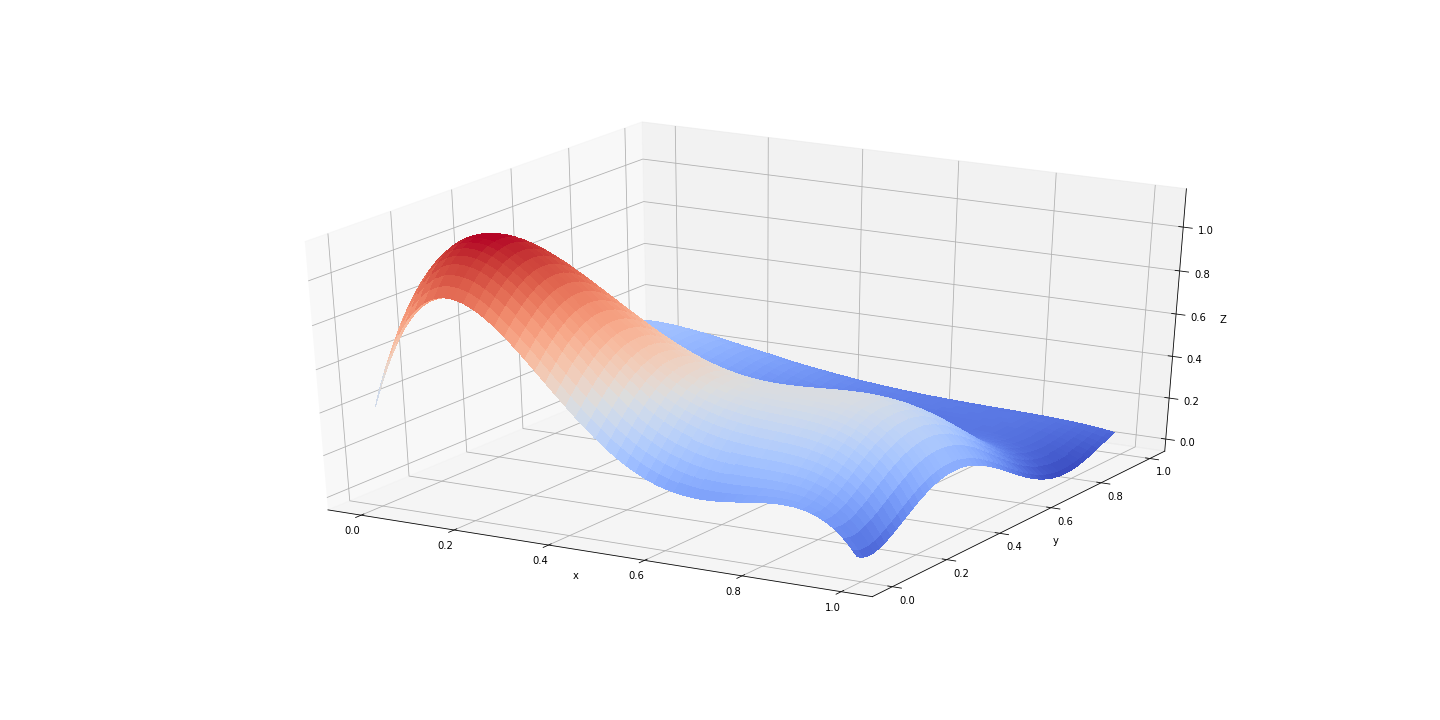
\includegraphics[width=1\textwidth]{figures/olsFranke.png}
        \caption{Three-dimensional plot of the predicted values of the Franke’s function using the best OSL regression model.}
        \label{fig:olsFranke}
\end{figure}

\begin{figure}[H]
\centering
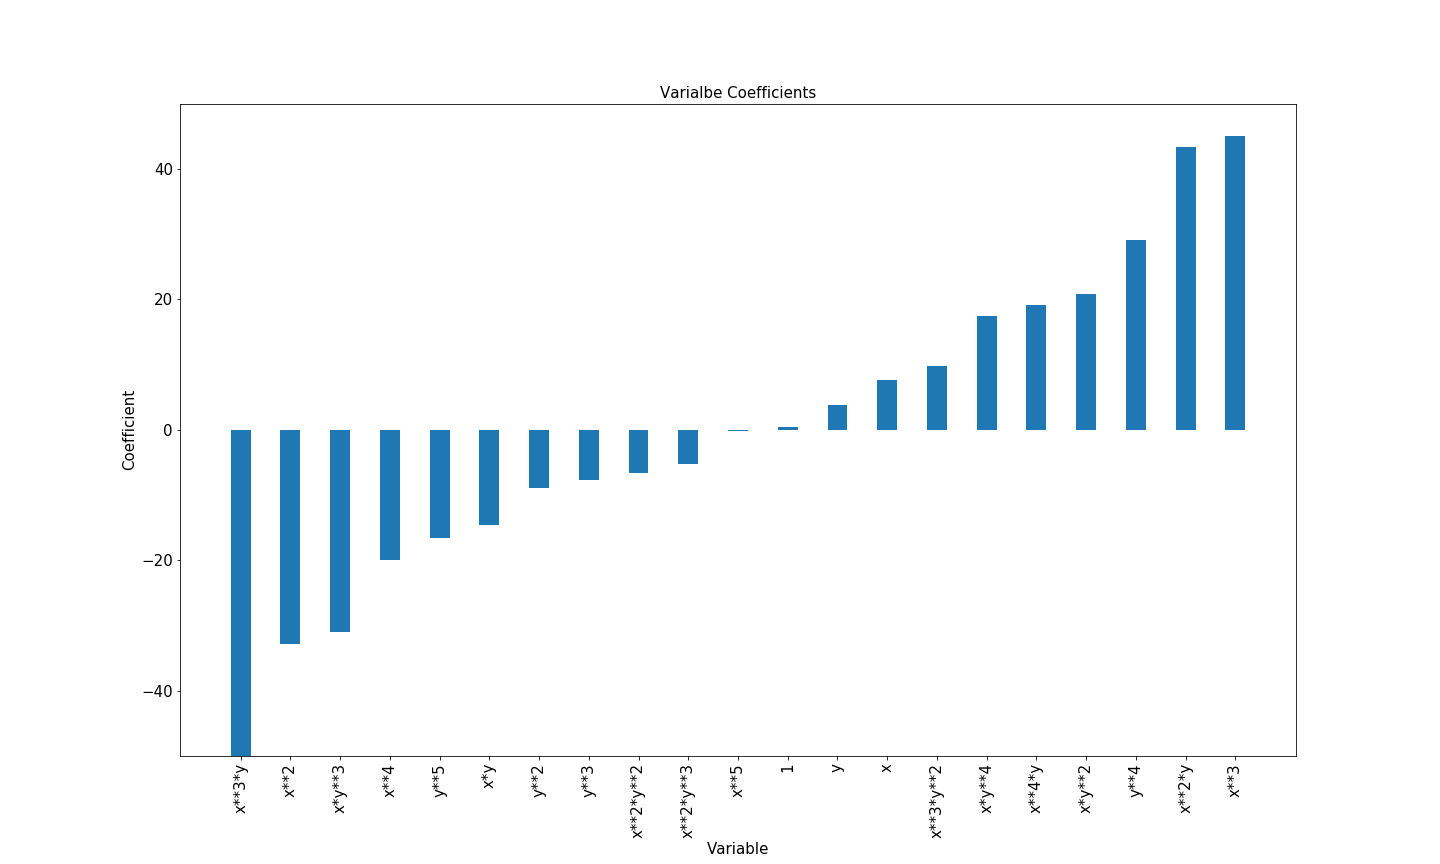
\includegraphics[width=1\textwidth]{figures/coeffOLS.png}
        \caption{Magnitudes of coefficients in the OLS model using polynomial approximation of order $5$.}
        \label{fig:coeffOLS}
\end{figure}

The magnitudes of coefficients in the final OLS model are illustrated in Figure \ref{fig:coeffOLS}. We see that the value of the Franke's function is more driven by terms $x^{3}$ and $x^{3}y$, since coefficients of these terms are much higher as compared to rest of the coefficients. It is important to note that the magnitudes of term $x^{5}$ and the intercept are relatively small, thus we could consider dropping these terms out of our model.\\
Whenever we discuss model prediction, it is important to understand prediction errors (bias and variance). Bias for the final model is: $0.00245$ and Variance is: $5.48e-07$. We conclude that our model is underfitted neither overfitted since the error of our model is relatively low. Finally, the three-dimensional plot of the predicted values of the Franke’s function is illustrated in figure \ref{fig:olsFranke}.


\subsubsection{Rigde regression on the Franke's function  with resampling}
In this part, we perform the same analysis as in the previous section for the Ridge regression with different values of $\alpha$ but now only with resampling.\\
As mentioned above our model is not overfitted, therefore it is not surprising that the best result is obtained using a low value of the tuning parameter $\alpha$. In Tables \ref{tab:ridge3}, \ref{tab:ridge4} and \ref{tab:ridge5} we see that as the value of $\alpha$ decreases the value of MSE for the Ridge regression model with resampling decreases, meanwhile the coefficient of determination $R^{2}$ is increasing.\\
Tables \ref{tab:ridge5} shows that the value of $R^{2}$ reaches the maximum at $\alpha=0.001$. In this case, the obtained results of the model using polynomial order $5$ is similar to the results using ordinary OLS model.
\begin{table}[H]
\centering
\begin{tabular}{lll}
\hline
$\alpha$ & MSE    & $R^{2}$ score \\ \hline
0.001     & 0.0082 & 0.90          \\
0.01      & 0.0082 & 0.90          \\
0.1       & 0.0082 & 0.90          \\
1         & 0.0102 & 0.87          \\
10        & 0.0161 & 0.80          \\
100       & 0.0235 & 0.71          \\ \hline
\end{tabular}
\caption{MSE and $R^{2}$ score of the Ridge regression model for the Franke's function using polynomials of order $3$.}
\label{tab:ridge3}
\end{table}

\begin{table}[H]
\centering
\begin{tabular}{lll}
\hline
$\alpha$ & MSE    & $R^{2}$ score \\ \hline
0.001     & 0.0043 & 0.94          \\
0.01      & 0.0047 & 0.94          \\
0.1       & 0.0071 & 0.91          \\
1         & 0.0091 & 0.88          \\
10        & 0.0137 & 0.83          \\
100       & 0.0223 & 0.73          \\ \hline
\end{tabular}
\caption{MSE and $R^{2}$ score of the Ridge regression model for the Franke's function using polynomials of order $4$.}
\label{tab:ridge4}
\end{table}

\begin{table}[H]
\centering
\begin{tabular}{lll}
\hline
$\alpha$ & MSE    & $R^{2}$ score \\ \hline
0.001     & 0.0027 & 0.96          \\
0.01      & 0.0037 & 0.95          \\
0.1       & 0.0056 & 0.93          \\
1         & 0.0089 & 0.89          \\
10        & 0.0124 & 0.85          \\
100       & 0.0213 & 0.74          \\ \hline
\end{tabular}
\caption{MSE and $R^{2}$ score of the Ridge regression model for the Franke's function using polynomials of order $5$.}
\label{tab:ridge5}
\end{table}

\begin{figure}[H]
\centering
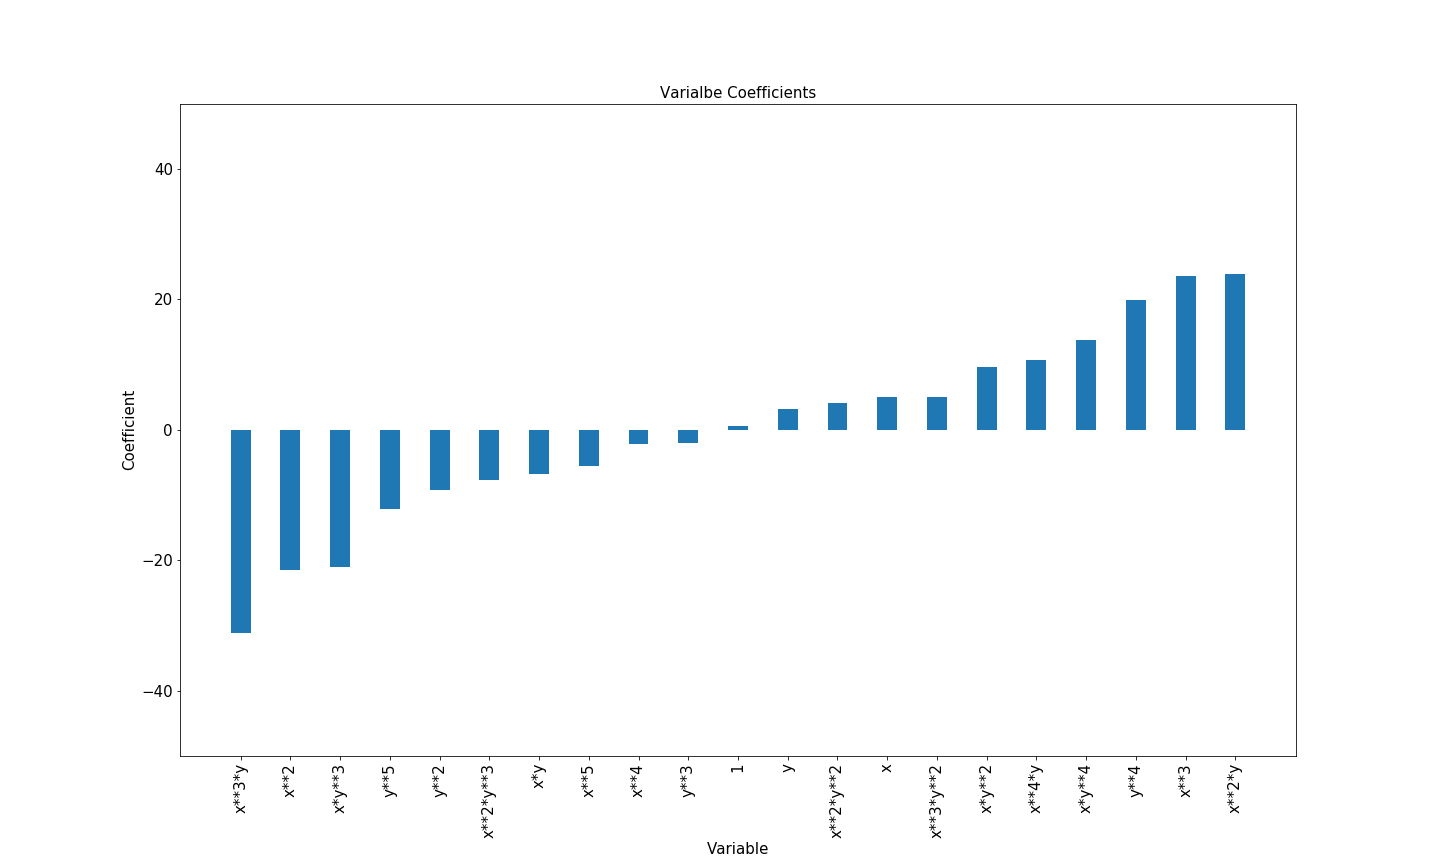
\includegraphics[width=1\textwidth]{figures/coeffRidge.png}
        \caption{Magnitudes of coefficients in the Ridge model using polynomial approximation of order $5$.}
        \label{fig:coeffRidge}
\end{figure}
In Figure \ref{fig:coeffRidge} we can see the effect of Ridge regression for $\alpha=0.001$, where the magnitudes of the coefficients in comparison with the OLS model have been decreased, also the values reach to zero but not absolute zero. Bias for the final Rigde model is: $0.00436$ and Variance: $8.61e-07$


\subsubsection{Lasso regression on the Franke's function  with resampling}
 
This part is essentially a repeat of the previous two ones, but now with Lasso regression with resampling. Tables \ref{tab:LassoFranke3}, \ref{tab:LassoFranke4} and \ref{tab:LassoFranke5} illustrate the results for Ridge regression using different values of $\alpha$ and orders of polynomials.\\
It is worth mentioning that for some values of $\alpha$ the coefficient of determination $R^{2}$ is negative. The reason is that by increasing $\alpha$ we reduce the magnitude of the coefficients. The higher the values of alpha, the bigger the penalty and therefore the magnitudes of coefficients are reduced more. For instance, in Figure \ref{fig:coeffLasso} we can see that even at small values of $\alpha=0.001$, the magnitudes of coefficients have reduced a lot.\\
However, we also know that our OLS model is not overfitted, which means that all predictors in our model are important and by reducing the magnitude of their coefficients we get worse predictions. 


\begin{table}[H]
\centering
\begin{tabular}{lll}
\hline
$\alpha$ & MSE    & $R^{2}$ score \\ \hline
0.001     & 0.0180 & 0.78          \\
0.01      & 0.0254 & 0.69          \\
0.1       & 0.0830 & -0.0011       \\
1         & 0.0830 & -0.0011       \\
10        & 0.0830 & -0.0011       \\
100       & 0.0830 & -0.0011       \\ \hline
\end{tabular}
\caption{MSE and $R^{2}$ score of the Lasso regression model for the Franke's function using polynomials of order $3$.}
\label{tab:LassoFranke3}
\end{table}

\begin{table}[H]
\centering
\begin{tabular}{lll}
\hline
$\alpha$ & MSE    & $R^{2}$ score \\ \hline
0.001     & 0.0142 & 0.82          \\
0.01      & 0.0254 & 0.69          \\
0.1       & 0.0830 & -0.0011       \\
1         & 0.0830 & -0.0011       \\
10        & 0.0830 & -0.0011       \\
100       & 0.0830 & -0.0011       \\ \hline
\end{tabular}
\caption{{MSE and $R^{2}$ score of the Lasso regression model for the Franke's function using polynomials of order $4$.}}
\label{tab:LassoFranke4}
\end{table}

\begin{table}[H]
\centering
\begin{tabular}{lll}
\hline
$\alpha$ & MSE    & $R^{2}$ score \\ \hline
0.001     & 0.0135 & 0.83          \\
0.01      & 0.0254 & 0.69          \\
0.1       & 0.0830 & -0.0011       \\
1         & 0.0830 & -0.0011       \\
10        & 0.0830 & -0.0011       \\
100       & 0.0830 & -0.0011       \\ \hline
\end{tabular}
\caption{MSE and $R^{2}$ score of the Lasso regression model for the Franke's function using polynomials of order $5$.}
\label{tab:LassoFranke5}
\end{table}

\begin{figure}[H]
\centering
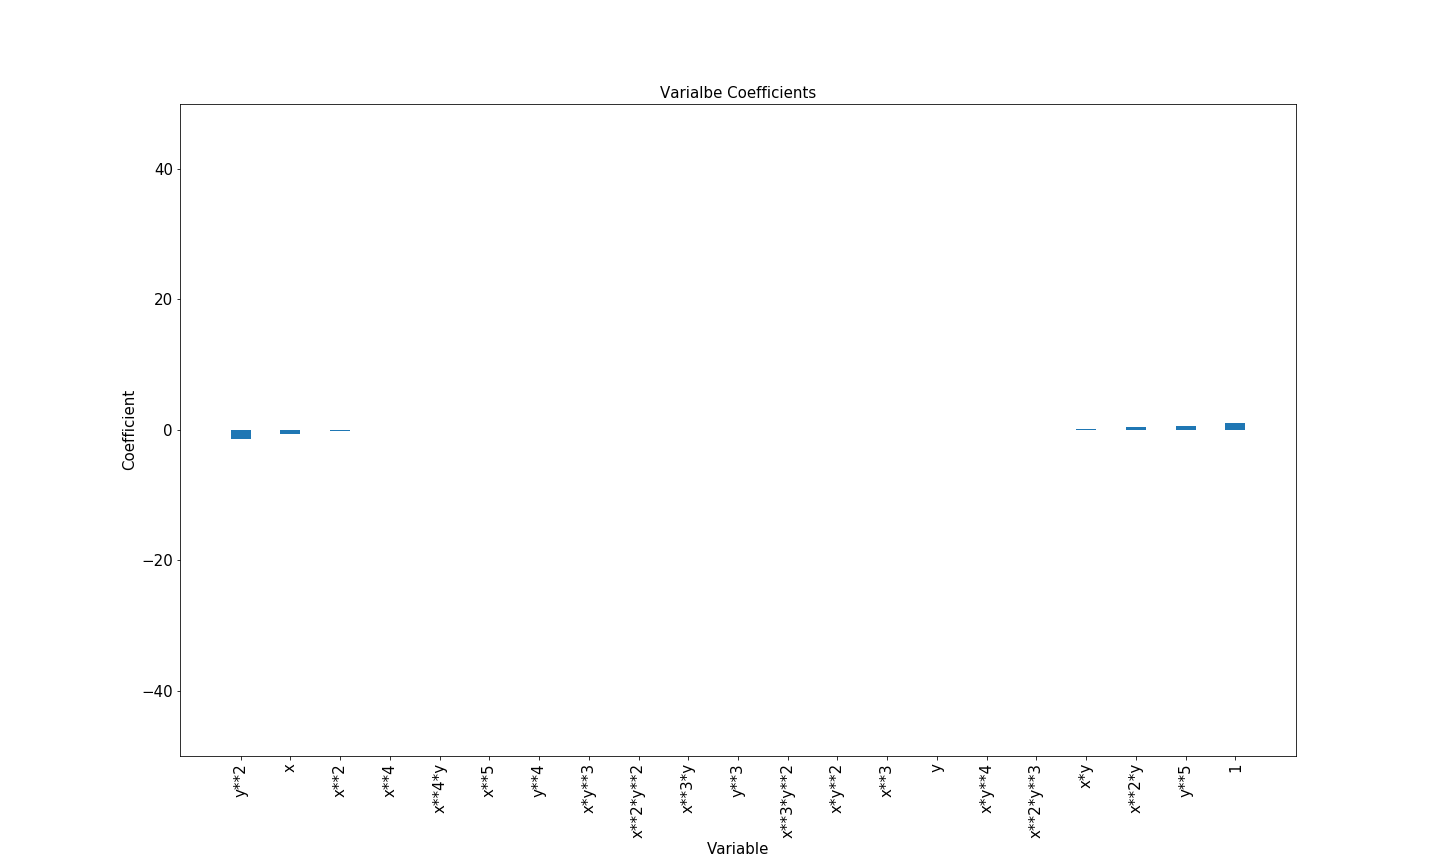
\includegraphics[width=1\textwidth]{figures/coeffLasso.png}
        \caption{Magnitudes of coefficients in the Lasso model using polynomial approximation of order $5$.}
        \label{fig:coeffLasso}
\end{figure}

Bias for the best Lasso model is $0.01349$ and Variance is $7.373e-07$. We can see that the value for the bias of the Lasso model has been increased in comparison with the OLS and Ridge model. Therefore, in this case, the Lasso model is predicting worse than both OLS and Ridge models.

\subsection{Real data}
\label{sec:realdata}
To illustrate the techniques described in Section \ref{sec:techniques}, we apply them to a digital terrain data from the website: https://earthexplorer.usgs.gov/. Figure \ref{fig:TerrainPrague} displays an image of the digital terrain data from Prague in the Czech Republic on a $2D$ regular raster. \\

\begin{figure}[H]
\centering
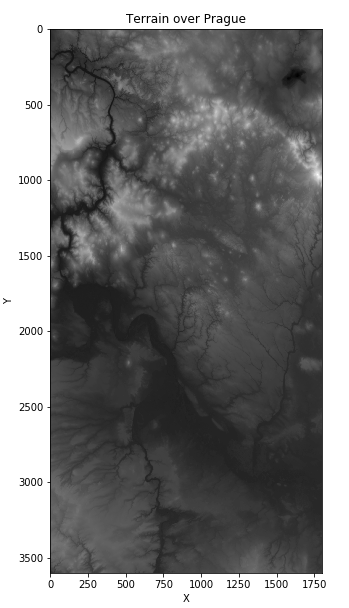
\includegraphics[width=0.5\textwidth]{figures/TerrainPrague.png}
        \caption{$2D$ image of the digital terrain data from Prague in Czech Republic.}
        \label{fig:TerrainPrague}
\end{figure}
As can be seen, the scale of this data set is much bigger than in the case of the Franke's function, therefore it is useful here to shrink the amount of data. In the next section, we divide our data set into $900$ smaller parts containing $120 \times 60$ data points. Next, we perform the same analysis as in the previous exercise for each part. The evaluation score that we use to measure the performance of presented models, such as MSE, $R^{2}$ etc., are computed by averaging the evaluation score derived in all parts. \\
%In next section, we apply all three methods for linear regression as in Section \ref{sebsec:franke}, the same %type of polynomial approximation and the same resampling techniques to evaluate which model fits the data best.
\subsubsection{OLS on the real data}
Regarding the performance of the OLS method, we present the results for the terrain data in Table \ref{tab:olsTerrain}. We see that the model using polynomials order $5$ outperformed the others, with almost twice as low MSE in comparison with the polynomial of order $3$ (170.80 vs 305.03). The $R^{2}$ score is $0.82$ for the highest order polynomial approximation and only $0.71$ for the lowest. 
\begin{table}[H]
\centering
\begin{tabular}{lll}
\hline
  & MSE    & R2 score \\ \hline
3 & 305.03 & 0.71      \\
4 & 219.98 & 0.78     \\
5 & 170.80 & 0.82     \\ \hline
\end{tabular}
\caption{MSE and $R^{2}$ score of the OSL regression model for the terrain data using polynomials of different orders.}
\label{tab:olsTerrain}
\end{table}

\begin{figure}[H]
\centering
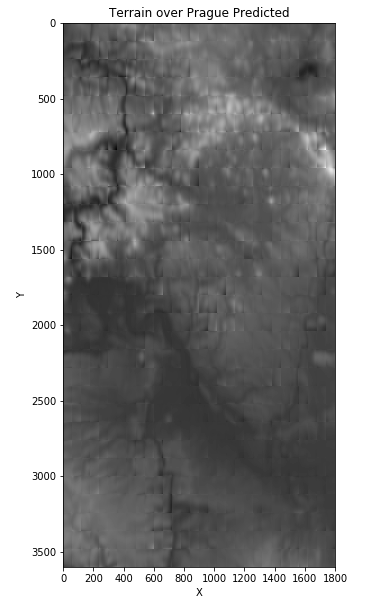
\includegraphics[width=0.5\textwidth]{figures/TerrainPraguePred.png}
        \caption{$2D$ image of the predicted terrain data from Prague using OSL regression model with polynomial approximation of order $5$.}
        \label{fig:TerrainPraguePred}
\end{figure}
In Figure \ref{fig:TerrainPraguePred} the image of the predicted terrain data is illustrated. Its obvious from the image that the reconstruction of the original image is not satisfactory. The comparison further shows that the average bias for the final model is: $169.51$ and the average variance is: $0.111$, which indicates that our model might be underfitted. We conclude that using a more complex model might help to reduce the bias.


\subsubsection{Ridge regression on the real data}
In Table \ref{tab:ridge5Terrain} we present the results for the terrain data using Ridge regression with polynomial approximation order $5$. Results for the remaining polynomial approximation can be found in the Appendix. Again, we see that as the value of $\alpha$ decreases the value of MSE for the Ridge regression model with K-folds cross-validation decreases, meanwhile the coefficient of determination $R^{2}$ is increasing.\\
Not surprisingly, the MSE is $170.65$ when using Ridge model with $\alpha=0.001$ which is very close to the number for the OLS model ($170.80$). A similar conclusion can be made for the $R^{2}$ score. The reason is that form the previous part we suspect that our model using polynomial approximation order $5$ might be underfitted, therefore by reducing magnitudes of the coefficients, only worse  results can be expected. Finally, the average bias for the final Rigde model is $169.51$ and the average variance is $0.102$.


\begin{table}[H]
\centering
\begin{tabular}{lll}
\hline
$\alpha$ & MSE    & $R^{2}$ score \\ \hline
0.001     & 170.65 & 0.82          \\
0.01      & 170.65 & 0.82          \\
0.1       & 170.65 & 0.82         \\
1         & 171.38 & 0.81          \\
10        & 209.01 & 0.70          \\
100       & 443.66 & 0.01          \\ \hline
\end{tabular}
\caption{MSE and $R^{2}$ score of the Ridge regression model for the terrain data using polynomials of order $5$.}
\label{tab:ridge5Terrain}
\end{table}


\subsubsection{Lasso regression on the real data}
Even worse is the performance of the model using Lasso regression using polynomial approximation order $5$, as can be seen in Table \ref{tab:ridge5Terrain}. Interestingly, the values of both MSE and $R^{2}$ score are very similar for all values of $\alpha$. The average bias for the Ridge model is $245.95$ and average variance is $0.086$.
\begin{table}[H]
\centering
\begin{tabular}{lll}
\hline
$\alpha$ & MSE    & $R^{2}$ score \\ \hline
0.001     & 246.98 & 0.76          \\
0.01      & 246.95 & 0.76          \\
0.1       & 246.93 & 0.76         \\
1         & 246.87 & 0.75          \\
10        & 251.73 & 0.75          \\
100       & 261.97 & 0.74          \\ \hline
\end{tabular}
\caption{MSE and $R^{2}$ score of the Lasso regression model for the terrain data using polynomials of order $5$.}
\label{tab:ridge5Terrain}
\end{table}


\section*{Conclusion}
In this text, we presented three different regression methods for data analysis. First, we introduced a very simple strategy which minimizes the sum of the squares of the differences between the observed dependent variable and those predicted by the model. Then, we presented more sophisticated methods which penalize the number of features in a model in order to only keep the most important features in the model. Next, k-fold cross-validation technique was introduced to perform a proper assessment of the presented techniques.\\
\\
At the beginning of the application part, the Franke's function was used to illustrate the presented methods. This was then followed by the analysis of the methods used on the real terrain data. To summarize, the OLS model has worked better for the Franke's function yielding lower MSE values and higher values of the $R^{2}$ score. We also conclude that neither the Ridge nor Lasso model offer clearly better results compared to the case when the OLS method is used. In our opinion, this is attributable to the simplicity of the model while using regularization. In the case of the terrain data, after reducing the magnitude of the coefficient, the model was not complex enough to accurately capture relationships between a dataset’s features and a target variable.  \\
\\
Furthermore, in the case of the terrain data, a deviation of the predicted values from the observed dependent variable for all models was quite large, resulting in a large value of error. The reason is that we represent an image as a vector and therefore we lose information about the vicinity of pixels. The reason is that the pixels which are close to each other could be very distant in the vector. Another point to note that inverting matrix for very large input vectors can be computationally expensive. Therefore we conclude that using classical regression techniques for larger data sets might be very unpractical.\\
\\
As part of the future expansion of this text, it would be desirable to implement some adaptive techniques for selecting the tuning parameter $\alpha$ used in regularization. We also should spend some more effort in researching a more effective approach to capture spatial relations between pixels in an image.

\newpage
\begin{thebibliography}{111}
\raggedright
\bibitem{abc} Christopher M. Bishop, Pattern Recognition and Machine Learning, Springer.
\bibitem{def} MARSLAND, Stephen. Machine learning: an algorithmic perspective. Chapman and Hall/CRC.
\bibitem{TRJ} Trevor Hastie, Robert Tibshirani, Jerome H. Friedman, The Elements of Statistical Learning. Springer
\bibitem{berkeley} Daniel Genk, Shannon Shih, Machine Learning Crash Course: Part 4 - The Bias-Variance Dilemma, https://ml.berkeley.edu/blog/2017/07/13/tutorial-4/
\bibitem{kfolds} Jason Brownlee, A Gentle Introduction to k-fold Cross-Validation, https://machinelearningmastery.com/k-fold-cross-validation/
\bibitem{2018arXiv180308823M} Mehta, P., Bukov, M., Wang, C.-H., et al., A high-bias, low-variance introduction to Machine Learning for physicists, arXiv:1803.08823 
\end{thebibliography}

\newpage
\appendix
\section{Appendix}
\begin{figure}[H]
\centering
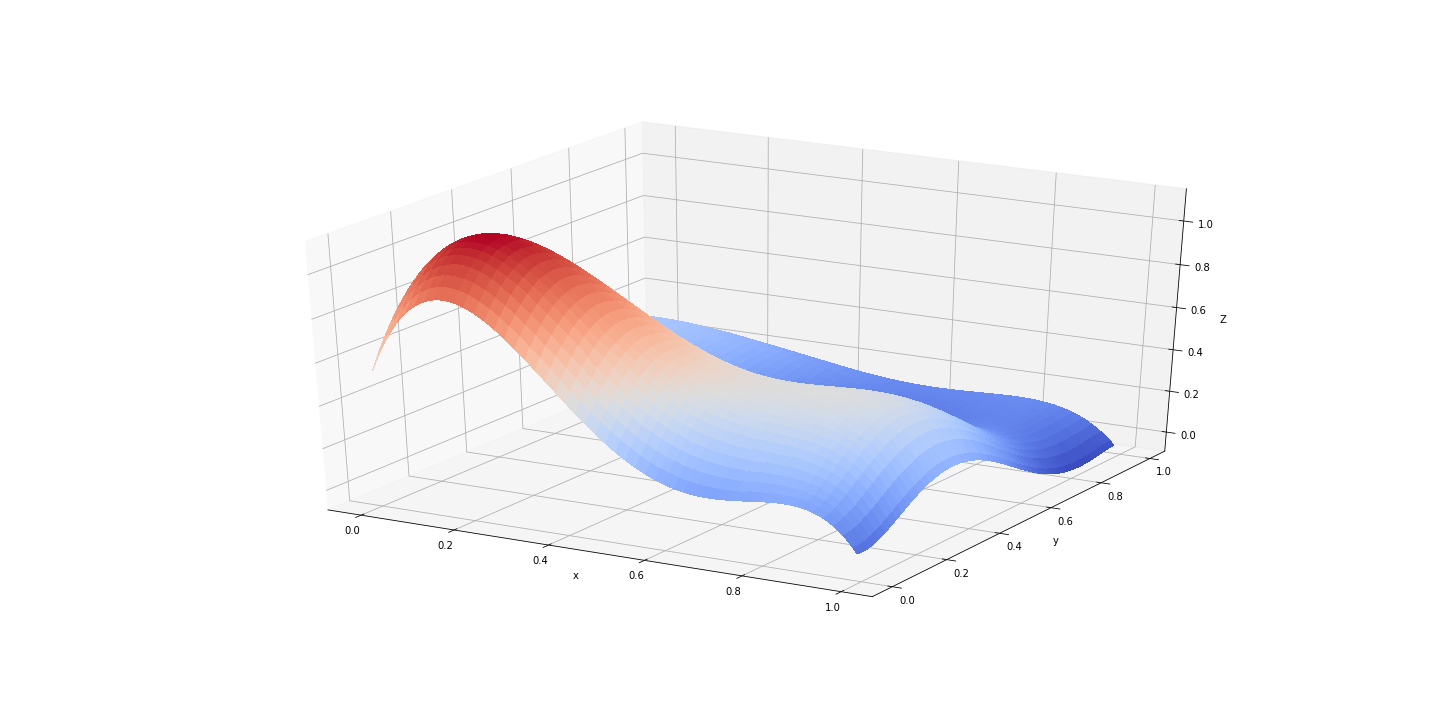
\includegraphics[width=1\textwidth]{figures/RidgeFranke.png}
        \caption{Three-dimensional plot of the predicted values of the Franke’s function using the best Ridge regression model.}
        \label{fig:RidgeFranke}
\end{figure}

\begin{figure}[H]
\centering
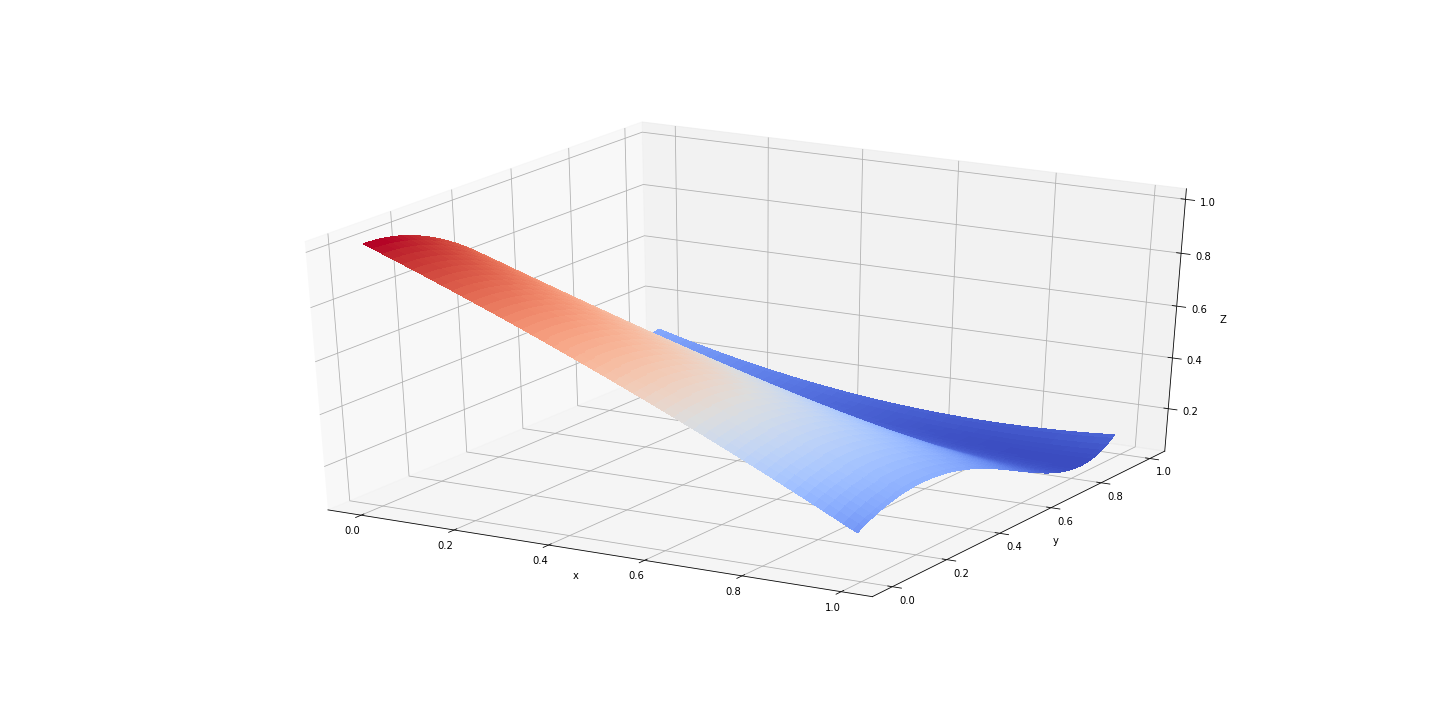
\includegraphics[width=1\textwidth]{figures/LassoFranke.png}
        \caption{Three-dimensional plot of the predicted values of the Franke’s function using the best Lasso regression model.}
        \label{fig:LassoFranke}
\end{figure}
\begin{table}[H]
\centering
\begin{tabular}{lll}
\hline
$\alpha$ & MSE    & $R^{2}$ score \\ \hline
0.001     & 304.89 & 0.71          \\
0.01      & 304.89 & 0.71          \\
0.1       & 304.89 & 0.71         \\
1         & 305.09 & 0.71         \\
10        & 321.40 & 0.66          \\
100       & 760.59 & -0.53          \\ \hline
\end{tabular}
\caption{MSE and $R^{2}$ score of the Ridge regression model for the terrain data using polynomials of order $3$.}
\label{tab:ridge3Terrain}
\end{table}

\begin{table}[H]
\centering
\begin{tabular}{lll}
\hline
$\alpha$ & MSE    & $R^{2}$ score \\ \hline
0.001     & 219.86 & 0.78          \\
0.01      & 219.86 & 0.78          \\
0.1       & 219.86 & 0.78         \\
1         & 220.27 & 0.78          \\
10        & 248.02 & 0.69          \\
100       & 599.39 & -0.31          \\ \hline
\end{tabular}
\caption{MSE and $R^{2}$ score of the Ridge regression model for the terrain data using polynomials of order $4$.}
\label{tab:ridge4Terrain}
\end{table}
\end{document}




